\subsection{Permutace}
\label{ssec:permutace}

Permutace jsou vlastně zobrazení, která prohazují prvky množin. Jejich asi
hlavním účelem je formalizovat koncept, že \uv{nezáleží na pořadí} nebo naopak,
že všechno dělám pro všechna možná přeuspořádání prvků. Člověk by měl dobrý
důvod si myslet, že nejsou dobré k ničemu jinému, než ke zkrášlení zápisu. Opak
je pravdou. Permutace mají velmi překvapivé aplikace v oblastech matematiky, kde
by je jeden nehledal. Zmiňme tři příklady.
\begin{itemize}
 \item Důkaz základní věty algebry -- tvrzení, že každý komplexní polynom má
  komplexní kořen -- silně využívá tzv. rozklad na symetrické polynomy, založený
  na vlastnostech permutací.
 \item Fakt, že kořeny obecných reálných (i komplexních) polynomů nelze zapsat v
  radikálech (tj. odmocninách), když je stupeň polynomu větší nebo roven 5 (tj.
  objevuje se v něm $x^{5}$), se opírá o tzv. \uv{neřešitelnost} permutačních
  grup (množin permutací na dané množině s binární operací skládání).
 \item Důkaz, že na každé Riemannově pseudovarietě dimenze 4 (kterou fyzikové
  používají jako model časoprostoru) existuje nekonečně mno\-ho neisomorfních
  Riemannových metrik (tj. v našem vesmíru mohu měřit vzdálenost nekonečně mnoha
  neekvivalentními způsoby) staví na symetrii tensorů definovaných pomocí
  permutací.
\end{itemize}

Takže, o co tu vlastně jde.
\begin{definition}[Permutace]
 \label{def:permutace}
 Bijekce $\sigma:X \to X$ konečné množiny $X$ na sebe samu se nazývá
 \emph{permutace} množiny $X$.

 Množinu všech permutací na $X$ značíme $S_X$ (jako grupa \textbf{s}ymetrií
 $X$). 
\end{definition}

Jelikož všichni rádi počítáme (xD), určíme si na začátek počet všech permutací
na dané množině. Podle
\hyperref[ex:proste-iff-na]{cvičení~\ref*{ex:proste-iff-na}}, které jste
\emph{všichni} dělali, zobrazení na konečné množině $X$ je prosté právě tehdy,
když je na, tedy právě tehdy, když je bijektivní. Tento fakt nám pomůže s
důkazem následujícího tvrzení. Jen ještě jedna definice usnadňující zápis.

\begin{definition}[Faktoriál]
\label{def:faktorial}
 Pro přirozené číslo $n \in \N$ definujeme
 \[
  n! \coloneqq \prod_{i=0}^{n-1} n-i. 
 \]
 Výraz $n!$ čteme $n$ \emph{faktoriál}.
\end{definition}

\begin{claim}[Počet permutací na množině]
\label{prop:pocet-permutaci-na-mnozine}
 Ať $X$ je konečná množina. Pak $\# S_X = (\# X)!$.
\end{claim}

\begin{proof}
 Podle
 \hyperref[claim:pocet-prostych-zobrazeni]{tvrzení~\ref{claim:pocet-prostych-zobrazeni}},
 počet prostých zobrazení $A \to B$ je
 \[
  \prod_{i=0}^{\# A-1} \# B - i.  
 \]
 Když $A = B$, pak bijekce $A \to A$ jsou totéž, co prostá zobrazení $A \to A$.
 Tedy, všech bijekcí $A \to A$ (tj. všech permutací na $A$) je
 \[
  \prod_{i=0}^{\# A-1} \# A - i = (\# A)!.\qedhere 
 \]
\end{proof}

\subsubsection{Zápis permutací}
\label{sssec:zapis-permutaci}

Budeme se chvíli bavit o tom, jak můžeme reprezentovat permutace. Samozřejmě,
permutace jsou mimo jiné zobrazení, takže je lze kreslit, jak už jsme to dělali;
tj. jako šipky mezi množinami teček.

Existují ale chytřejší a přehlednější způsoby, jak je znázornit. Jeden možný
způsob je zápisem do řádku. Řekněme, že $X = \{1,2,3,4\}$ a $\sigma \in S_X$.
Když napíšeme, že
\[
 \sigma = 
 \begin{pmatrix}
  1 & 2 & 3 & 4\\
  3 & 2 & 4 & 1
 \end{pmatrix},
\]
myslíme tím, že $\sigma$ je zobrazení, které posílá $1$ na $3$, $2$ na $2$, $3$
na $4$ a $4$ na $1$. Můžeme navíc předpokládat, že vrchní řádek je vždycky v
nějakém předem dohodnutém pořadí a permutaci $\sigma$ zapsat prostě jako
\[
 \sigma = \begin{pmatrix} 
 3 & 2 & 4 & 1
 \end{pmatrix}. 
\]
V obvyklém kreslení permutací bychom $\sigma$ znázornili, jak vidíte na 
\hyperref[fig:permutace-jako-sipky]{obrázku níže}.
\begin{figure}[h]
 \centering
 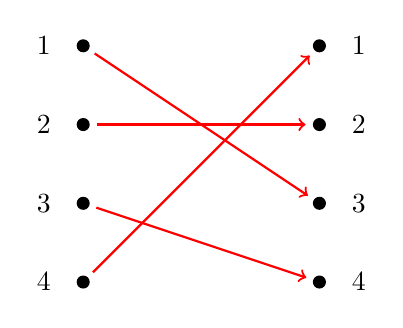
\begin{tikzpicture}
  \filldraw[black] (-1.5,0) circle (.5ex) {};
  \filldraw[black] (-1.5,1) circle (.5ex) {};
  \filldraw[black] (-1.5,2) circle (.5ex) {};
  \filldraw[black] (-1.5,3) circle (.5ex) {};
  \node at (-2, 0) {$4$};
  \node at (-2, 1) {$3$};
  \node at (-2, 2) {$2$};
  \node at (-2, 3) {$1$};

  \filldraw[black] (1.5,0) circle (.5ex) {};
  \filldraw[black] (1.5,1) circle (.5ex) {};
  \filldraw[black] (1.5,2) circle (.5ex) {};
  \filldraw[black] (1.5,3) circle (.5ex) {};
  \node at (2, 0) {$4$};
  \node at (2, 1) {$3$};
  \node at (2, 2) {$2$};
  \node at (2, 3) {$1$};

  \draw[thick,red,->,shorten <=5pt,shorten >=5pt] (-1.5, 3) -- (1.5, 1);
  \draw[thick,red,->,shorten <=5pt,shorten >=5pt] (-1.5, 2) -- (1.5, 2);
  \draw[thick,red,->,shorten <=5pt,shorten >=5pt] (-1.5, 1) -- (1.5, 0);
  \draw[thick,red,->,shorten <=5pt,shorten >=5pt] (-1.5, 0) -- (1.5, 3);
 \end{tikzpicture}
 \label{fig:permutace-jako-sipky}
 \caption{Permutace $\clr{\sigma}$ zakreslená šipkami.}
\end{figure}

Ačkoli je tento způsob zápisu intuitivní a podporuje představu permutace jako
\uv{proházení} prvků na množině, mnohem více se používá tzv. zápis v cyklech.
Důvody jsou primárně formální; z cyklického zápisu se velmi snadno totiž pozná,
jak \uv{řád} permutace, tak její rozložení na \uv{transpozi\-ce}. Oba pojmy
definujeme a vysvětlíme později.

Jelikož permutace jsou bijekce z množiny do téže množiny, můžeme vždy začít v
nějakém libovolné prvku a pokračovat po šipkách, dokud se nedostaneme opět na
ten samý prvek. Tento přístup formalizuje právě zápis do cyklů. Například
zápis permutace $\clr{\sigma} = (3\;2\;4\;1)$ do cyklů by vypadal takto:
\begin{figure}[h]
 \centering
 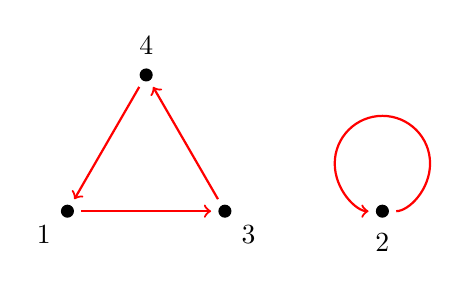
\begin{tikzpicture}
  \filldraw[black] (-1,0) circle (.5ex) {};
  \filldraw[black] (1,0) circle (.5ex) {};
  \filldraw[black] (0,1.73) circle (.5ex) {};

  \node at (-1.3, -0.3) {$1$};
  \node at (1.3, -0.3) {$3$};
  \node at (0, 2.1) {$4$};

  \filldraw[black] (3,0) circle (.5ex) {};
  \node at (3, -0.4) {$2$};

  \draw[thick,red,->,shorten <=5pt,shorten >=5pt] (-1, 0) -- (1, 0);
  \draw[thick,red,->,shorten <=5pt,shorten >=5pt] (1, 0) -- (0, 1.73);
  \draw[thick,red,->,shorten <=5pt,shorten >=5pt] (0, 1.73) -- (-1, 0);
  \draw[thick,red,->,shorten <=5pt,shorten >=5pt] (3, 0) arc (-90:270:4ex);
 \end{tikzpicture}
 \label{fig:permutace-jako-cyklus}
 \caption{Zápis permutace $\clr{\sigma}$ do cyklů.}
\end{figure}

Jak si asi dovedete představit, tento zápis znamená, že permutace $\clr{\sigma}$
pošle $1$ na $3$, pak $3$ na $4$ a nakonec $4$ na $1$. Tedy, po třech
\uv{iteracích} permutace $\clr{\sigma}$ se dostaneme z prvku $1$ opět do prvku
$1$. Smyčka nad $2$ samozřejmě znamená, že $2$ se zobrazuje opět na $2$.

Zápis na \hyperref[fig:permutace-jako-cyklus]{obrázku výše} je evidentně dosti
neúsporný, a v textu tudíž těžko použitelný. Obvykle se taková permutace zapíše
jako $\sigma = (134)(2)$. Tedy, jednotlivé cykly jsou odděleny závorkami a šipky
v cyklech vedou zleva doprava, případně z posledního prvku zpět na první.

Konečně, smyčky (tj. zobrazení prvku na sebe sama) se z cyklického zápisu běžně
vynechávají. Svoji oblíbenou permutaci $\sigma = (134)(2)$ můžeme proto úplně
nejúsporněji zapsat jako $\sigma = (134)$. Zápis permutací v cyklech budeme
odteď využívat výhradně.

\begin{warning}
 Zápis permutace pomocí cyklů \textbf{není jednoznačný}. Je to pro to, že u
 daného cyklu nelze říct, kde \uv{končí} a kde \uv{začíná}. Důležité je pouze
 pořadí prvků. Permutace $(134), (341)$ a $(413)$ jsou tudíž jedna a ta samá.
\end{warning}

\subsubsection{Skládání permutací}
\label{sssec:skladani-permutaci}

Jelikož permutace jsou speciálně zobrazení, dají se pochopitelně skládat. Navíc,
protože doména i kodoména každé permutace na $X$ je právě množina $X$, mohu je
skládat v libovolném pořadí a libovolném množství.

Na výpočet složení dvou permutací $\sigma,\tau \in S_X$ není myslím žádný
vyloženě snadný postup. Člověk se musí zkrátka v cyklickém zápisu dočíst, kam
posílá první permutace daný prvek, a kam zase druhá permutace posílá obraz
tohoto prvku.

\begin{example}
 Ať $X = \{1,2,3,4\}$ a $\sigma,\tau \in S_X, \sigma = (134), \tau = (14)(23)$.
 Pak
 \[
  \sigma\tau = (243),
 \]
 protože $\tau$ pošle $1$ na $4$ a $\sigma$ pošle $4$ na $1$, tedy  $\sigma\tau$
 pošle $1$ na $1$. Podobně pro ostatní prvky. Dále,
 \[
  \tau\sigma = (123).
 \]
\end{example}
\begin{warning}
 Jak bylo vidno z předchozího příkladu, skládání permutací (jako obecně i
 relací) \textbf{není komutativní}. Dokonce platí, že pouze skládání permutace
 se sebou samou je komutativní, čili jsou-li $\sigma,\tau \in S_X$
 \[
  \sigma\tau = \tau\sigma \implies \tau = \sigma
 \]
 za předpokladu, že $\# X \geq 3$.
\end{warning}
